\documentclass[11pt,a4paper]{article} %% 1.Ebene = chapter, headings

\usepackage[utf8]{inputenc} 
\usepackage[T1]{fontenc} 
\usepackage{lmodern}
\usepackage{tcolorbox}

\usepackage[german]{babel}


\setlength{\parindent}{0pt}
\setlength{\parskip}{1ex plus 0.5ex minus 0.5ex}

\usepackage{amsmath} 


\usepackage{graphicx} 

\usepackage[section]{placeins}
\usepackage{booktabs}


\usepackage{hyperref}
\hypersetup{
	colorlinks,
	citecolor=red,
	filecolor=black,
	linkcolor=black,
	urlcolor=black}
\graphicspath{}

\begin{document}



{
	\centering 
	\large 
	Physiklabor für Anfänger*innen \\
	Ferienpraktikum im Sommersemester 2018 \\[4mm]
	\textbf{\LARGE 
		Versuch 22: Kreiselpräzession
	} \\[3mm]
	(durchgeführt am 21.09.2018 bei Adrian Hauber) \\
	Ye Joon Kim, Marouan Zouari\\
	\today \\[10mm]
}

\section{Einführung}
Ein schräger Kreisel, auf den eine Gravitationskraft wirkt, führt eine Präzession aus, da das auf den Kreisel wirkenden Drehmoment verursacht eine Änderung des Drehmoments senkrecht zur Kraft und Figurenachse. 


\section{Ziel des Versuchs}
Das Ziel dieses Versuchs ist es, das Trägheitsmoment des Kreisels entlang der Figurenachse durch die Messung der Präzessions- und Rotationsgeschwindigkeiten zu bestimmen.

\section{Aufbau}

\section{Durchführung}

\section{Auswertung und Fehleranalyse}
Zur Bestimmung des Trägheitsmoments entlang der Figurenachse wird die oben hergeleitete Formel benutzt, nämlich:
$$I_A = \frac{rG}{\omega_F \omega_P}$$

Zuerst wurden die Werte für $\omega_F$ und $\omega_P$ für die verschiedene $x$ und Messreihen bestimmt (Siehe Anhang 1). 
\begin{tcolorbox}[colback=white]
\subsubsection{Rechenweg}
Für die Bestimmung von $\omega$ wurde die folgende Formel benutzt:
$$ \omega = \frac{T_\textrm{Tot}}{n}\frac{1}{2\pi}$$
Wobei $T_\textrm{Tot}$ die gesamte Zeitdauer der Messung, und $n$ die Anzahl Drehungen war.
Für den Fehler wurde der Messfehler durch $sqrt{n}$ geteilt, da es handelt sich um einen Mittelwert.
\end{tcolorbox}

Um den Offset zwischen $x$, der Skala auf der Kreiselachse, und $r$, der Abstand zwischen den Schwerpunkt und Unterstützungspunkt zu bestimmen wurde $\frac{\omega_F\omega_P}{G}$ gegen $x$ aufgetragen. Da $I_A$ eine Konstante ist, muss $\omega_P$ bei $r = 0$ unendlich sein. Deswegen in einem Plot von $\frac{\omega_F\omega_P}{G}$ gegen $x$ soll es eine Unstetigkeitsstelle geben. Der $x$ Wert von dieser Unstetigkeitsstelle ist dann das Offset zwischen $x$ und $r$ (Siehe Abbildung 1).
\begin{tcolorbox}[colback=white] 
\subsubsection{Rechenweg}
Zuerst wurden die Werte für $\frac{\omega_F\omega_P}{G}$ für alle Messreihen berechnet. Die Fehler für $\frac{\omega_F\omega_P}{G}$ wurden mit der Formel für die Standardabweichung bestimmt, nämlich:
$$s_x = \sqrt{\frac{\sum_{i=1}^{n}(x_i-\bar{x})^2}{n-1}} $$
\end{tcolorbox}

\begin{figure}
	\centering
	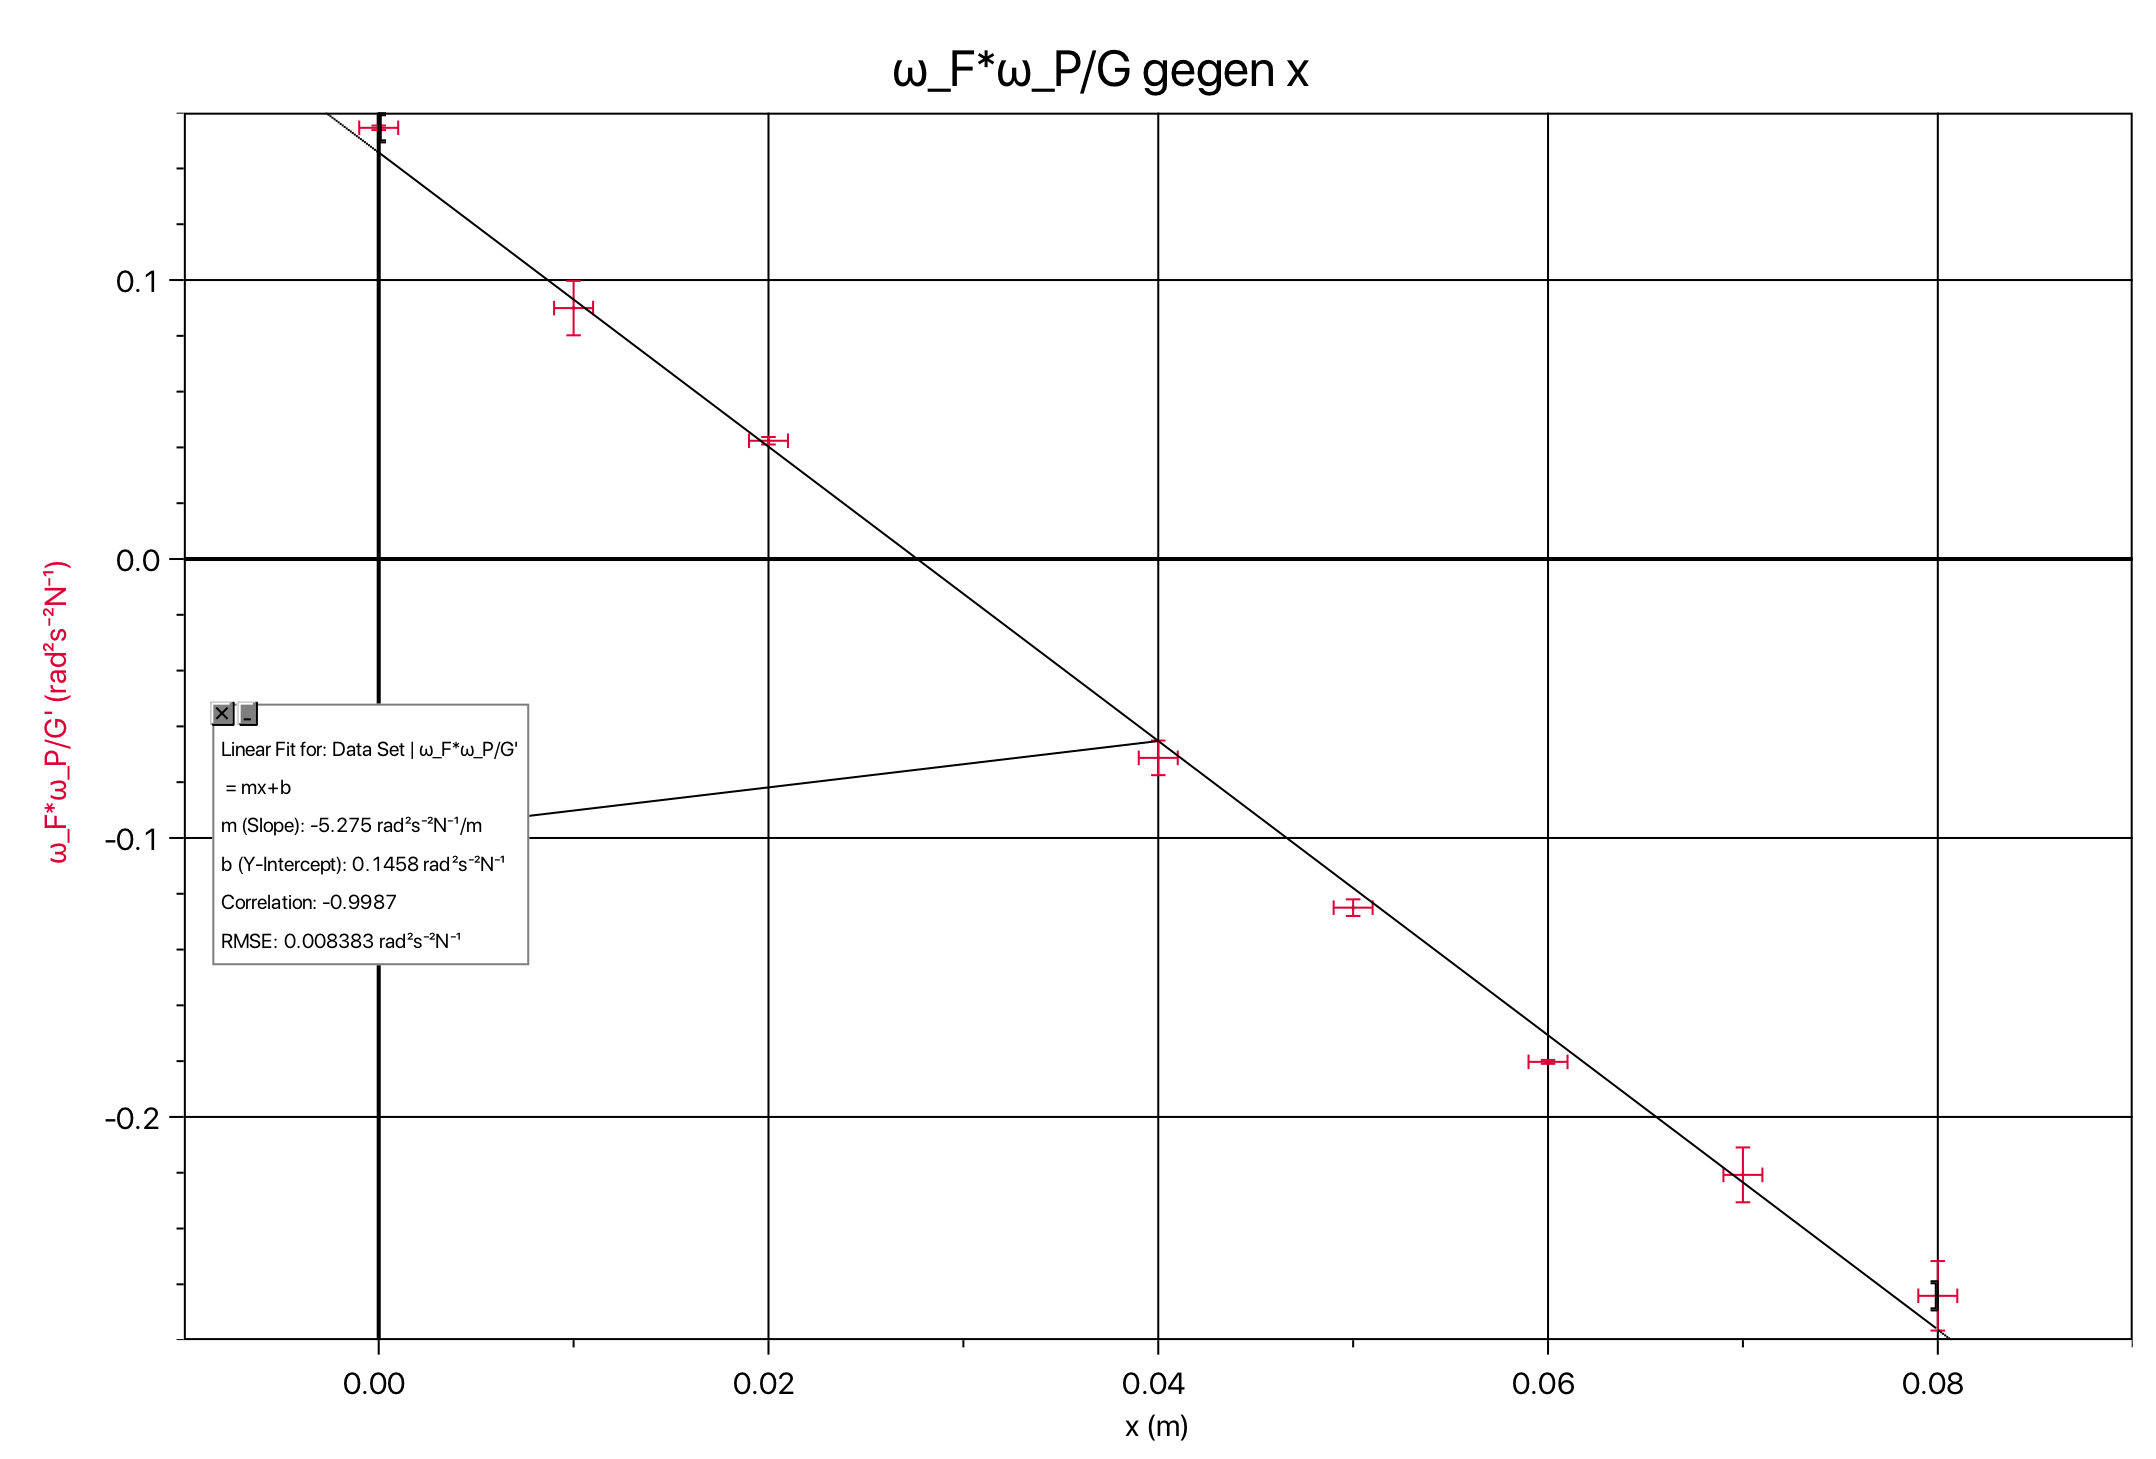
\includegraphics[width=\linewidth]{Abb1}
	\caption{$\frac{\omega_F\omega_P}{G}$ als Funktion von der Position $x$}
\end{figure}

Angenommen, dass der Verlauf etwas wie Abbildung (2) aussieht, kann es abgeschätzt werden, dass die Unstetigkeitsstelle ungefähr bei $x=0,03$m liegt. Das wurde auch experimentell bestätigt, da bei $x=0,03$ schient es so, als gäbe es keine Präzession. Der Fehler wurde als 0,002 m abgeschätzt. die Werte für $x$ kann jetzt in $r$ umgerechnet werden (Siehe Tabelle 1). 

\begin{figure}
	\centering
	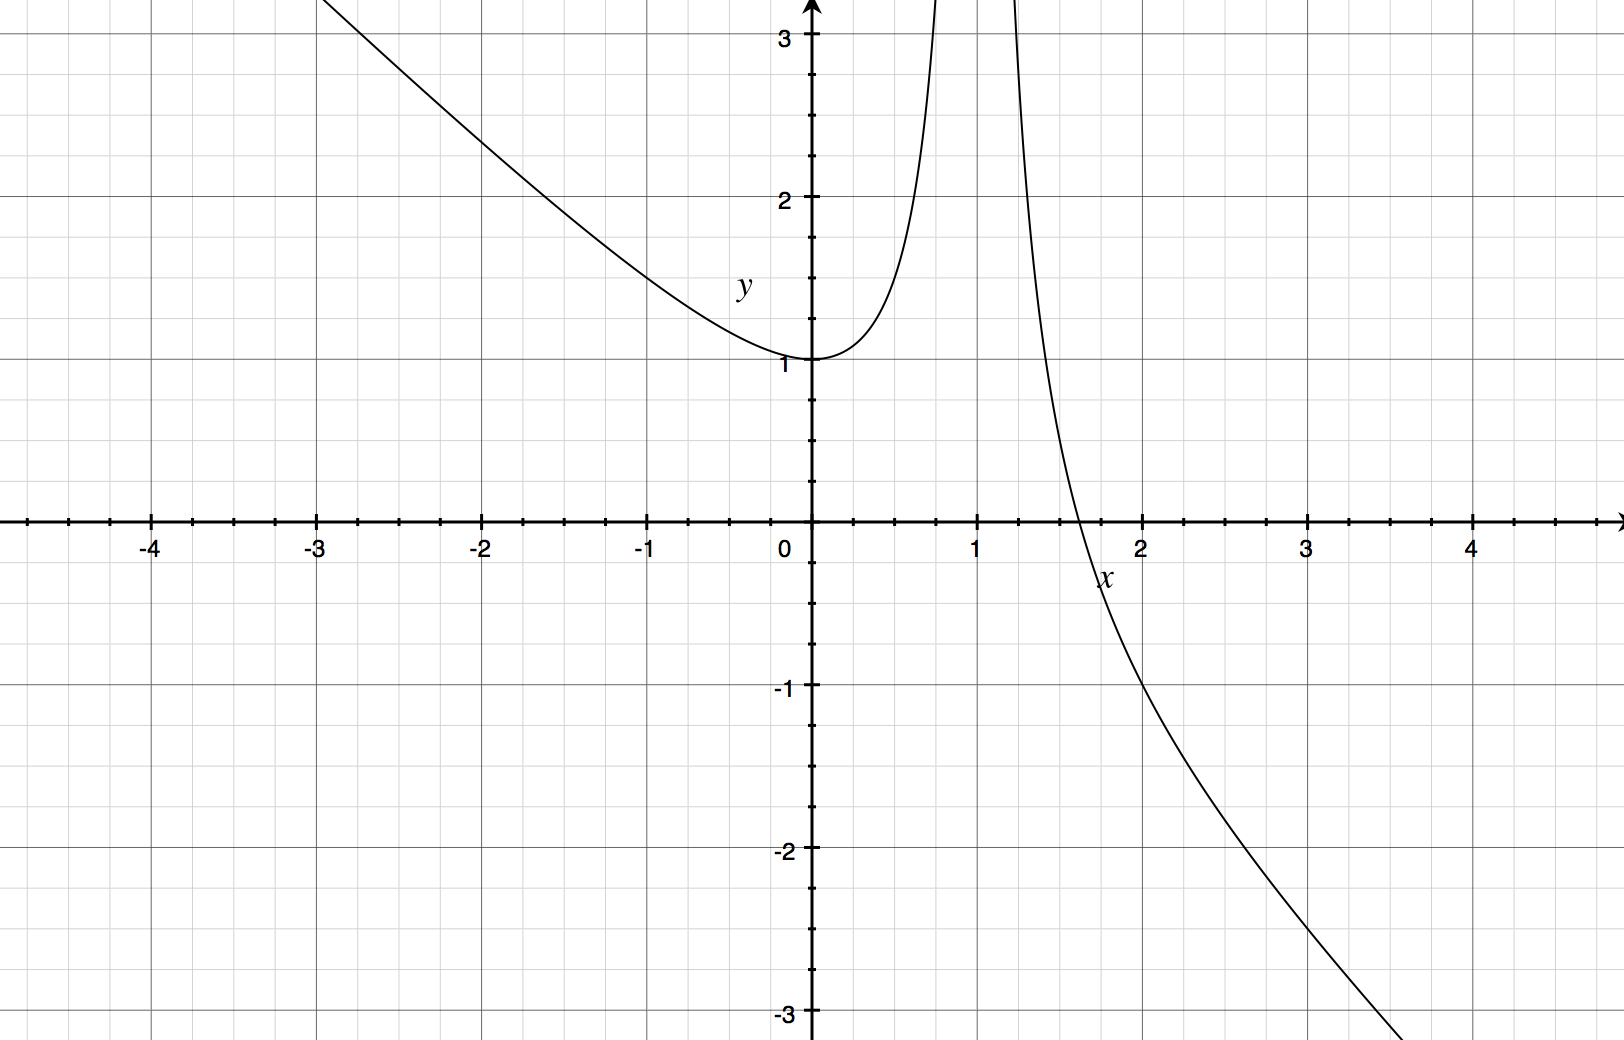
\includegraphics[width=\linewidth]{Abb2}
	\caption{Eine Beispielfunktion}
\end{figure}

\begin{table}[h]
	\centering
	\begin{tabular*}{0.15\textwidth}{@{\extracolsep{\fill}}rr}
		\toprule
		\multicolumn{1}{c}{$x$} & \multicolumn{1}{c}{$r$}\\
		\multicolumn{1}{c}{m} & \multicolumn{1}{c}{m} \\
		\midrule
		0 &  0,03\\
		0,01 &  0,02\\
		0,02 &  0,01\\
		0,04 & -0,01\\
		0,05 & -0,02\\
		0,06 & -0,03\\
		0,07 & -0,04\\ 
		0,08 & -0,05\\
		\bottomrule
	\end{tabular*}
	\caption{Umrechnung von $x$ auf $r$}
	\label{tabelle}
\end{table}

$\frac{\omega_F\omega_P}{G}$ wurde gegen $r$ geplottet. In diesem Fall entspricht die Steigung dem Wert für $\frac{1}{I_A}$, da die Formel für $I_A$ lässt sich umformen als:
$$\frac{\omega_F\omega_P}{G} = \frac{1}{I_A}r$$ 
Mit einem Microsoft-Excel Dokument wurde die lineare Regression und die Fehlerrechnungen durchgeführt. 

\section{Diskussion der Ergebnisse}

\section{Literatur}

\section{Anhang}

\begin{table}[h]
	\centering
	\begin{tabular*}{0.99\textwidth}{@{\extracolsep{\fill}}cccccc}
		\toprule
		x & Messreihe & $\omega_F$ & $u_{\omega_F}$ & $\omega_P$ & $u_{\omega_P}$ \\
		m &  &    \\
		\bottomrule
		0 & 1 & 0,46 & 0,06 & 10,8 & 0,2 \\
		& 2 & 0,50 & 0,06 & 9,9 & 0,2 \\
		 & 3 & 0,47 & 0,06 & 10,5 & 0,2 \\
		0,01 & 1 & 0,56 & 0,06 & 17,3 & 0,3\\
		& 2 & 0,69 & 0,06 & 11,8 & 0,3 \\
		& 3 & 0,51 & 0,06 & 15,7 & 0,3 \\
		0,02 & 1 & 0,48 & 0,06 & 36,0  &  0,3\\
		& 2 & 0,48 &0,06 & 38,4 & 0,3  \\
		& 3 & 0,46 & 0,06 & 40,1 & 0,3 \\
		0,04 & 1 & 0,50 & 0,06 & 23,1&0,3 \\
		& 2 & 0,58 &0,06&18,8&0,3 \\
		& 3 & 0,52 &0,06&18,7&0,3 \\
		0,05 & 1 & 0,47 &0,06&13,2&0,2 \\
		& 2 & 0,43&0,06&13,9&0,2 \\
		& 3 & 0,42&0,06&14,8&0,2 \\
		0,06 & 1 & 0,44 & 0,06 &9,7&0,2 \\
		& 2 & 0,50 & 0,06&8,5&0,2 \\
		& 3 & 0,49 & 0,05&9,6&0,2 \\
		0,07 & 1 & 0,43 &0,06&8,3&0,3 \\
		& 2 & 0,50&0,06&6,6&0,3 \\
		& 3 & 0,48&0,06&7,3&0,3 \\
		0,08 & 1 & 0,47 & 0,06&6,2&0,3 \\
		& 2 & 0,50 & 0,06&6,0&0,3 \\
		& 3 & 0,53&0,06&5,2&0,3 \\
		\bottomrule
	\end{tabular*}
	\caption{Die Berechnete Winkelgeschwindigkeiten für Präzession und Rotation bei verschiedene $x$}
	\label{tabelle}
\end{table}
(Unsicherheiten der $x$ sind 0,001m)
\end{document}